% !TEX encoding = UTF-8
% !TEX TS-program = pdflatex
% !TEX root = ../tesi.tex
% !TEX spellcheck = it-IT

%**************************************************************
\chapter{Casi d'uso secondari}
%**************************************************************

\hypertarget{UC3}{}
\section{Caso d'uso UC3: gestione user}

        \begin{figure}[H]
            \centering
            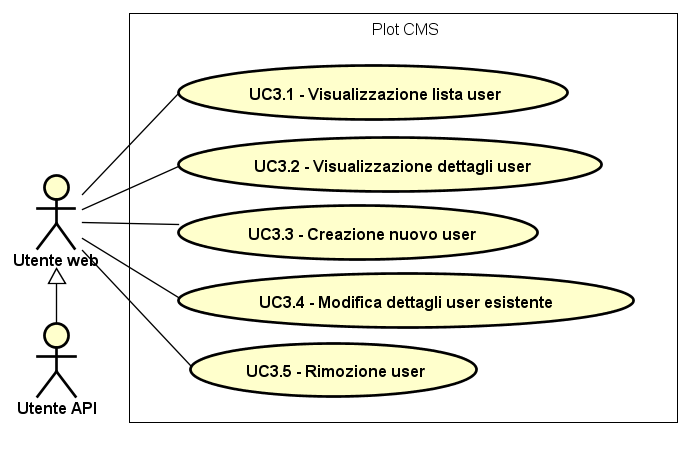
\includegraphics[scale=0.95, width=\textwidth]{immagini/usecase/UC3.png}
            \caption{Caso d'uso UC3: gestione user}\label{fig:UC3} 
        \end{figure}
\begin{itemize}
\item \textbf{Attori}: utente web, utente API;
\item \textbf{Descrizione}: un utente autenticato deve poter gestire gli aspetti di base legati agli utenti del gioco: creazione, visualizzazione, modifica e rimozione; 
      \item \textbf{Precondizione}: l'utente accede alla piattaforma attraverso un browser web o attraverso le API REST esposte dal sistema;

        \item \textbf{Flusso principale degli eventi}:
          \begin{enumerate}
          \item L'utente autenticato può visualizzare la lista degli utenti del gioco;
          \item L'utente autenticato può visualizzare i dettagli di uno specifico utente del gioco (\hyperlink{UC3.2}{UC3.2});
          \item L'utente autenticato può creare un nuovo utente del gioco (\hyperlink{UC3.3}{UC3.3});
          \item L'utente autenticato può modificare i dettagli di uno specifico utente di gioco (\hyperlink{UC3.4}{UC3.4});
          \item L'utente autenticato può rimuovere un utente del gioco.

      \end{enumerate}
    \item \textbf{Postcondizione}: il sistema ha erogato le funzionalità richieste dall'utente.
  \end{itemize}

\hypertarget{UC3.2}{}
\section{Caso d'uso UC3.2: visualizzazione dettagli user}
\begin{itemize}
\item \textbf{Attori}: utente web, utente API;
\item \textbf{Descrizione}: l'utente autenticato deve poter visualizzare i dettagli relativi ad uno specifico utente del gioco; 
      \item \textbf{Precondizione}: l'utente accede alla piattaforma attraverso un browser web o attraverso le API REST esposte dal sistema. L'utente del gioco che si vuole visualizzare deve esistere;

        \item \textbf{Flusso principale degli eventi}:
          \begin{enumerate}
          \item L'utente autenticato visualizza il nome dell'utente di gioco;
          \item L'utente autenticato visualizza il cognome dell'utente di gioco;
          \item L'utente autenticato visualizza l'email dell'utente di gioco;
          \item L'utente autenticato visualizza l'ambito lavorativo dell'utente di gioco;
          \item L'utente autenticato visualizza la regione di appartenenza dell'utente di gioco;
          \item L'utente autenticato visualizza la lingua preferita dell'utente di gioco;
          \item L'utente autenticato visualizza il team dell'utente di gioco.

      \end{enumerate}
    \item \textbf{Postcondizione}: il sistema mostra all'utente i dettagli dell'utente del gioco richiesto.
  \end{itemize}
\hypertarget{UC3.3}{}
\section{Caso d'uso UC3.3: creazione nuovo user}
\begin{itemize}
\item \textbf{Attori}: utente web, utente API;
\item \textbf{Descrizione}: l'utente autenticato deve poter creare un nuovo utente del gioco; 
      \item \textbf{Precondizione}: l'utente accede alla piattaforma attraverso un browser web o attraverso le API REST esposte dal sistema;

        \item \textbf{Flusso principale degli eventi}:
          \begin{enumerate}
          \item L'utente autenticato inserisce il nome dell'utente del gioco;
          \item L'utente autenticato inserisce il cognome dell'utente del gioco;
          \item L'utente autenticato inserisce l'indirizzo email dell'utente del gioco;
          \item L'utente autenticato può inserire la password dell'utente del gioco;
          \item L'utente autenticato può inserire l'ambito lavorativo dell'utente del gioco;
          \item L'utente autenticato può inserire la regione d'appartenenza dell'utente del gioco;
          \item L'utente autenticato può inserire la lingua preferita dell'utente del gioco;
          \item L'utente autenticato può inserire il team dell'utente del gioco.

      \end{enumerate}
    \item \textbf{Postcondizione}: il sistema crea un nuovo utente del gioco e ne mostra i dettagli all'utente.
  \end{itemize}
	
\hypertarget{UC3.4}{}
\section{Caso d'uso UC3.4: modifica dettagli user esistente}
\begin{itemize}
\item \textbf{Attori}: utente web, utente API;
\item \textbf{Descrizione}: l'utente autenticato deve poter modificare i dettagli relativi ad un utente del gioco esistente; 
      \item \textbf{Precondizione}: l'utente accede alla piattaforma attraverso un browser web o attraverso le API REST esposte dal sistema. L'utente del gioco che si vuole modificare deve esistere;

        \item \textbf{Flusso principale degli eventi}:
          \begin{enumerate}
          \item L'utente autenticato può modificare il nome dell'utente del gioco;
          \item L'utente autenticato può modificare il cognome dell'utente del gioco;
          \item L'utente autenticato può modificare l'indirizzo email dell'utente del gioco;
          \item L'utente autenticato può modificare l'ambito lavorativo dell'utente del gioco;
          \item L'utente autenticato può modificare la regione di appartenenza dell'utente del gioco;
          \item L'utente autenticato può modificare la lingua preferita dell'utente del gioco;
          \item L'utente autenticato può modificare il team di appartenenza dell'utente del gioco;
          \item L'utente autenticato può modificare il team di appartenenza dell'utente del gioco;
          \item L'utente autenticato può modificare il team di appartenenza dell'utente del gioco.

      \end{enumerate}
    \item \textbf{Postcondizione}: il sistema apporta le modifiche richieste e mostra i dettagli dell'utente di gioco modificato all'utente autenticato.
  \end{itemize}
\hypertarget{UC4}{}
\section{Caso d'uso UC4: gestione team}

        \begin{figure}[H]
            \centering
            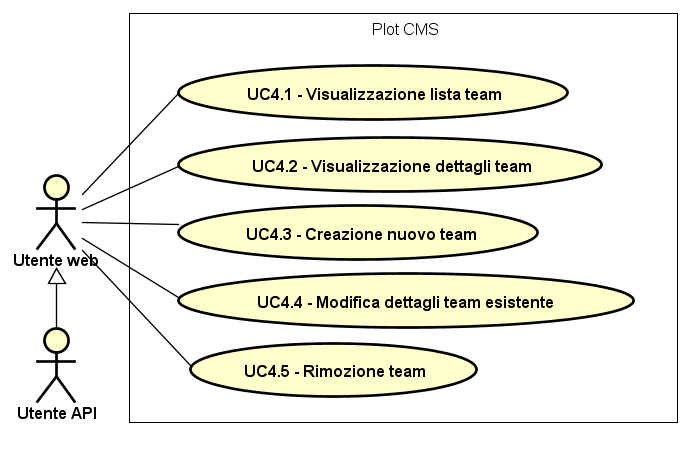
\includegraphics[scale=0.95, width=\textwidth]{immagini/usecase/UC4.png}
            \caption{Caso d'uso UC4: gestione team}\label{fig:UC4} 
        \end{figure}
\begin{itemize}
\item \textbf{Attori}: utente web, utente API;
\item \textbf{Descrizione}: un utente autenticato deve poter gestire gli aspetti di base legati ai team: creazione, visualizzazione, modifica e rimozione; 
      \item \textbf{Precondizione}: l'utente accede alla piattaforma attraverso un browser web o attraverso le API REST esposte dal sistema;

        \item \textbf{Flusso principale degli eventi}:
          \begin{enumerate}
          \item L'utente autenticato può visualizzare la lista dei team (\hyperlink{UC4.1}{UC4.1});
          \item L'utente autenticato può visualizzare i dettagli di uno specifico team (\hyperlink{UC4.2}{UC4.2});
          \item L'utente autenticato può creare un team (\hyperlink{UC4.3}{UC4.3});
          \item L'utente autenticato può modificare i dettagli di uno specifico team (\hyperlink{UC4.4}{UC4.4});
          \item L'utente autenticato può rimuovere un team (\hyperlink{UC4.5}{UC4.5}).

      \end{enumerate}
    \item \textbf{Postcondizione}: il sistema ha erogato le funzionalità richieste dall'utente.
  \end{itemize}
\hypertarget{UC4.1}{}
\section{Caso d'uso UC4.1: visualizzazione lista team}
\begin{itemize}
\item \textbf{Attori}: utente web, utente API;
\item \textbf{Descrizione}: l'utente autenticato deve poter visualizzare una lista di tutti i team in gioco. Ogni team deve riportare il numero di componenti e il punteggio totale, ovvero la somma dei punteggi ottenuti nelle mission disputate; 
      \item \textbf{Precondizione}: l'utente autenticato accede alla piattaforma attraverso un browser web o attraverso le API REST esposte dal sistema;

        \item \textbf{Flusso principale degli eventi}:
          \begin{enumerate}
          \item L'utente autenticato visualizza la lista dei team in gioco.

      \end{enumerate}
    \item \textbf{Postcondizione}: il sistema mostra la lista dei team in gioco.
  \end{itemize}
\hypertarget{UC4.2}{}
\section{Caso d'uso UC4.2: visualizzazione dettagli team}
\begin{itemize}
\item \textbf{Attori}: utente web, utente API;
\item \textbf{Descrizione}: l'utente autenticato deve poter visualizzare i dettagli relativi ad uno specifico team in gioco; 
      \item \textbf{Precondizione}: l'utente accede alla piattaforma attraverso un browser web o attraverso le API REST esposte dal sistema. Il team che si vuole visualizzare deve esistere;

        \item \textbf{Flusso principale degli eventi}:
          \begin{enumerate}
          \item L'utente autenticato visualizza il nome del team;
          \item L'utente autenticato visualizza l'URL dell'immagine rappresentativa del team;
          \item L'utente autenticato visualizza la lista degli utenti del gioco appartenenti al team.

      \end{enumerate}
    \item \textbf{Postcondizione}: il sistema mostra all'utente i dettagli del team richiesto.
  \end{itemize}
\hypertarget{UC4.3}{}
\section{Caso d'uso UC4.3: creazione nuovo team}
\begin{itemize}
\item \textbf{Attori}: utente web, utente API;
\item \textbf{Descrizione}: l'utente autenticato deve poter creare un nuovo team di gioco; 
      \item \textbf{Precondizione}: l'utente accede alla piattaforma attraverso un browser web o attraverso le API REST esposte dal sistema;

        \item \textbf{Flusso principale degli eventi}:
          \begin{enumerate}
          \item L'utente autenticato inserisce il nome del team;
          \item L'utente autenticato può inserire l'URL di un'immagine rappresentativa del team.

      \end{enumerate}
    \item \textbf{Postcondizione}: il sistema crea un nuovo team e ne mostra i dettagli all'utente.
  \end{itemize}
\hypertarget{UC4.4}{}
\section{Caso d'uso UC4.4: modifica dettagli team esistente}
\begin{itemize}
\item \textbf{Attori}: utente web, utente API;
\item \textbf{Descrizione}: l'utente autenticato deve poter modificare i dettagli relativi ad un team esistente; 
      \item \textbf{Precondizione}: l'utente accede alla piattaforma attraverso un browser web o attraverso le API REST esposte dal sistema. Il team che si vuole modificare deve esistere;

        \item \textbf{Flusso principale degli eventi}:
          \begin{enumerate}
          \item L'utente autenticato può modificare il nome del team;
          \item L'utente autenticato può modificare l'URL dell'immagine rappresentativa del team.

      \end{enumerate}
    \item \textbf{Postcondizione}: il sistema apporta le modifiche richieste e mostra i dettagli del team modificato all'utente.
  \end{itemize}
\hypertarget{UC4.5}{}
\section{Caso d'uso UC4.5: rimozione team}
\begin{itemize}
\item \textbf{Attori}: utente web, utente API;
\item \textbf{Descrizione}: l'utente autenticato deve poter rimuovere un team di gioco; 
      \item \textbf{Precondizione}: l'utente autenticato accede alla piattaforma attraverso un browser web o attraverso le API REST esposte dal sistema. Il team che si vuole rimuovere deve esistere;

        \item \textbf{Flusso principale degli eventi}:
          \begin{enumerate}
          \item L'utente autenticato rimuove un particolare team di gioco	.

      \end{enumerate}
    \item \textbf{Postcondizione}: Il team viene rimosso dal sistema e non può più essere recuperato. Il sistema mostra all'utente una lista degi team ancora presenti nel sistema.
  \end{itemize}
\hypertarget{UC5}{}
\section{Caso d'uso UC5: gestione admin}

        \begin{figure}
            \centering
            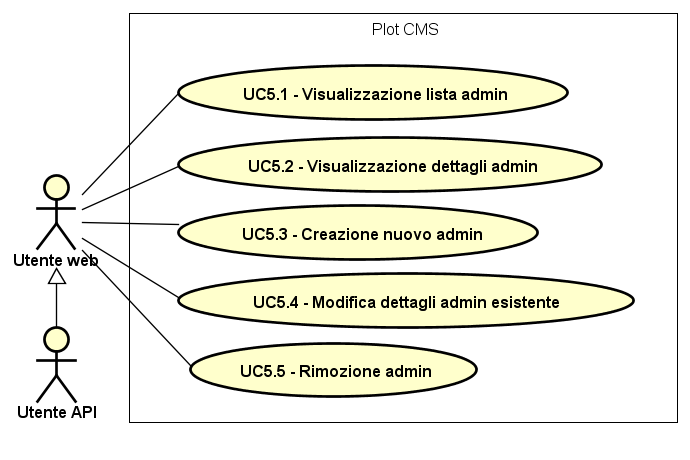
\includegraphics[scale=0.95, width=\textwidth]{immagini/usecase/UC5.png}
            \caption{Caso d'uso UC5: gestione admin}\label{fig:UC5} 
        \end{figure}
\begin{itemize}
\item \textbf{Attori}: utente web, utente API;
\item \textbf{Descrizione}: un utente autenticato deve poter gestire gli aspetti di base legati agli amministratori della piattaforma: creazione, visualizzazione, modifica e rimozione; 
      \item \textbf{Precondizione}: l'utente accede alla piattaforma attraverso un browser web o attraverso le API REST esposte dal sistema;

        \item \textbf{Flusso principale degli eventi}:
          \begin{enumerate}
          \item L'utente autenticato può visualizzare la lista degli amministratori della piattaforma (\hyperlink{UC5.1}{UC5.1});
          \item L'utente autenticato può visualizzare i dettagli di uno specifico amministratore della piattaforma (\hyperlink{UC5.2}{UC5.2});
          \item L'utente autenticato può creare un nuovo amministratore della piattaforma (\hyperlink{UC5.3}{UC5.3});
          \item L'utente autenticato può modificare i dettagli di uno specifico amministratore della piattaforma (\hyperlink{UC5.4}{UC5.4});
          \item L'utente autenticato può rimuovere un amministratore della piattaforma (\hyperlink{UC5.5}{UC5.5}).

      \end{enumerate}
    \item \textbf{Postcondizione}: il sistema ha erogato le funzionalità richieste dall'utente.
  \end{itemize}
\hypertarget{UC5.1}{}
\section{Caso d'uso UC5.1: visualizzazione lista admin}
\begin{itemize}
\item \textbf{Attori}: utente web, utente API;
\item \textbf{Descrizione}: l'utente autenticato deve poter visualizzare una lista di tutti gli amministratori della piattaforma. Gli amministratori sono coloro che possono utilizzare le funzionalità offerte dalla piattaforma; 
      \item \textbf{Precondizione}: l'utente autenticato accede alla piattaforma attraverso un browser web o attraverso le API REST esposte dal sistema;

        \item \textbf{Flusso principale degli eventi}:
          \begin{enumerate}
          \item L'utente autenticato visualizza la lista degli amministratori della piattaforma.

      \end{enumerate}
    \item \textbf{Postcondizione}: il sistema mostra la lista degli amministratori della piattaforma.
  \end{itemize}
\hypertarget{UC5.2}{}
\section{Caso d'uso UC5.2: visualizzazione dettagli admin}
\begin{itemize}
\item \textbf{Attori}: utente web, utente API;
\item \textbf{Descrizione}: l'utente autenticato deve poter visualizzare i dettagli relativi ad uno specifico amministratore della piattaforma; 
      \item \textbf{Precondizione}: l'utente accede alla piattaforma attraverso un browser web o attraverso le API REST esposte dal sistema. L'amministratore che si vuole visualizzare deve esistere;

        \item \textbf{Flusso principale degli eventi}:
          \begin{enumerate}
          \item L'utente autenticato visualizza il nome dell'amministratore della piattaforma;
          \item L'utente autenticato visualizza il cognome dell'amministratore della piattaforma;
          \item L'utente autenticato visualizza l'email dell'amministratore della piattaforma.

      \end{enumerate}
    \item \textbf{Postcondizione}: il sistema mostra all'utente i dettagli dell'amministratore richiesto.
  \end{itemize}
\hypertarget{UC5.3}{}
\section{Caso d'uso UC5.3: creazione nuovo admin}
\begin{itemize}
\item \textbf{Attori}: utente web, utente API;
\item \textbf{Descrizione}: l'utente autenticato deve poter creare un nuovo amministratore della piattaforma ; 
      \item \textbf{Precondizione}: l'utente accede alla piattaforma attraverso un browser web o attraverso le API REST esposte dal sistema;

        \item \textbf{Flusso principale degli eventi}:
          \begin{enumerate}
          \item L'utente autenticato inserisce il nome dell'amministratore della piattaforma;
          \item L'utente autenticato inserisce il cognome dell'amministratore della piattaforma;
          \item L'utente autenticato inserisce l'email dell'amministratore della piattaforma;
          \item L'utente autenticato inserisce la password dell'amministratore della piattaforma.

      \end{enumerate}
    \item \textbf{Postcondizione}: il sistema crea un nuovo amministratore della piattaforma e ne mostra i dettagli all'utente.
  \end{itemize}
\hypertarget{UC5.4}{}
\section{Caso d'uso UC5.4: modifica dettagli admin esistente}
\begin{itemize}
\item \textbf{Attori}: utente web, utente API;
\item \textbf{Descrizione}: l'utente autenticato deve poter modificare i dettagli relativi ad un amministratore esistente; 
      \item \textbf{Precondizione}: l'utente accede alla piattaforma attraverso un browser web o attraverso le API REST esposte dal sistema. L'amministratore che si vuole modificare deve esistere;

        \item \textbf{Flusso principale degli eventi}:
          \begin{enumerate}
          \item L'utente autenticato può modificare il nome dell'amministratore;
          \item L'utente autenticato può modificare il cognome dell'amministratore;
          \item L'utente autenticato può modificare l'email dell'amministratore.

      \end{enumerate}
    \item \textbf{Postcondizione}: il sistema apporta le modifiche richieste e mostra i dettagli dell'amministratore modificato all'utente.
  \end{itemize}
\hypertarget{UC5.5}{}
\section{Caso d'uso UC5.5: rimozione admin}
\begin{itemize}
\item \textbf{Attori}: utente web, utente API;
\item \textbf{Descrizione}: l'utente autenticato deve poter rimuovere un amministratore della piattaforma; 
      \item \textbf{Precondizione}: l'utente autenticato accede alla piattaforma attraverso un browser web o attraverso le API REST esposte dal sistema. L'amministratore che si vuole rimuovere deve esistere;

        \item \textbf{Flusso principale degli eventi}:
          \begin{enumerate}
          \item L'utente autenticato rimuove un particolare amministratore della piattaforma.

      \end{enumerate}
    \item \textbf{Postcondizione}: l'amministratore viene rimosso dal sistema e non può più essere recuperato. Il sistema mostra all'utente una lista degli amministratori ancora presenti nel sistema.
  \end{itemize}
\hypertarget{UC6}{}
\section{Caso d'uso UC6: gestione log}

        \begin{figure}[H]
            \centering
            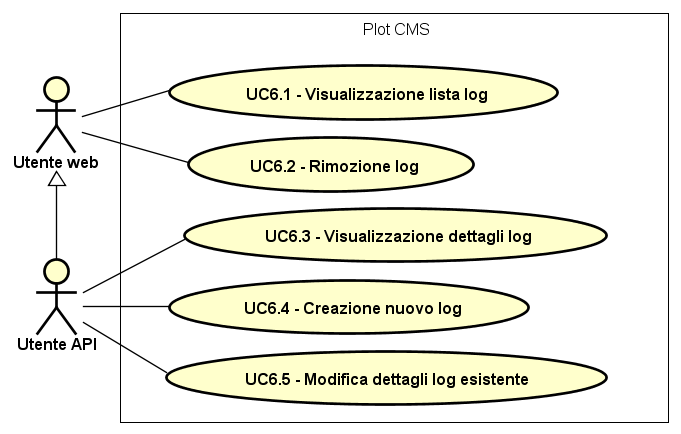
\includegraphics[scale=0.95, width=\textwidth]{immagini/usecase/UC6.png}
            \caption{Caso d'uso UC6: gestione log}\label{fig:UC6} 
        \end{figure}
\begin{itemize}
\item \textbf{Attori}: utente web, utente API;
\item \textbf{Descrizione}: un utente autenticato che accede alla piattaforma dal web deve poter gestire la visualizzazione e la rimozione dei log generati dagli utenti del gioco.
In aggiunta a ciò, un utente autenticato che accede alla piattaforma attraverso le API deve poter creare un nuovo log e modificare un log esistente; 
      \item \textbf{Precondizione}: l'utente accede alla piattaforma attraverso un browser web o attraverso le API REST esposte dal sistema;

        \item \textbf{Flusso principale degli eventi}:
          \begin{enumerate}
          \item L'utente autenticato che accede tramite web può visualizzare la lista dei log (\hyperlink{UC6.1}{UC6.1});
          \item L'utente autenticato che accede tramite web può rimuovere un log (\hyperlink{UC6.2}{UC6.2});
          \item L'utente autenticato che accede tramite API può visualizzare i dettagli di uno specifico log (\hyperlink{UC6.3}{UC6.3});
          \item L'utente autenticato che accede tramite API può creare un nuovo log (\hyperlink{UC6.4}{UC6.4});
          \item L'utente autenticato che accede tramite API può modificare i dettagli di uno specifico log (\hyperlink{UC6.5}{UC6.5}).

      \end{enumerate}
    \item \textbf{Postcondizione}: il sistema ha erogato le funzionalità richieste dall'utente.
  \end{itemize}
\hypertarget{UC6.1}{}
\section{Caso d'uso UC6.1: visualizzazione lista log}
\begin{itemize}
\item \textbf{Attori}: utente web, utente API;
\item \textbf{Descrizione}: l'utente autenticato deve poter visualizzare una lista di tutti i log generati dalle richieste HTTP effettuate dagli utenti di gioco ; 
      \item \textbf{Precondizione}: l'utente autenticato accede alla piattaforma attraverso un browser web o attraverso le API REST esposte dal sistema;

        \item \textbf{Flusso principale degli eventi}:
          \begin{enumerate}
          \item L'utente autenticato visualizza la lista dei log generati dalle richieste HTTP effettuate dagli utenti di gioco .

      \end{enumerate}
    \item \textbf{Postcondizione}: il sistema mostra la lista dei log generati dalle richieste HTTP effettuate dagli utenti di gioco .
  \end{itemize}
\hypertarget{UC6.2}{}
\section{Caso d'uso UC6.2: rimozione log}
\begin{itemize}
\item \textbf{Attori}: utente web, utente API;
\item \textbf{Descrizione}: l'utente autenticato deve poter rimuovere un log generato da una richiesta HTTP effettuata da un utente di gioco; 
      \item \textbf{Precondizione}: l'utente autenticato accede alla piattaforma attraverso un browser web o attraverso le API REST esposte dal sistema. Il log che si vuole rimuovere deve esistere;

        \item \textbf{Flusso principale degli eventi}:
          \begin{enumerate}
          \item L'utente autenticato rimuove un log generato da una richiesta HTTP effettuata da un utente di gioco.

      \end{enumerate}
    \item \textbf{Postcondizione}: il log viene rimosso dal sistema e non può più essere recuperato. Il sistema mostra all'utente una lista dei log ancora presenti nel sistema.
  \end{itemize}
\hypertarget{UC6.3}{}
\section{Caso d'uso UC6.3: visualizzazione dettagli log}
\begin{itemize}
\item \textbf{Attori}: utente API;
\item \textbf{Descrizione}: l'utente autenticato deve poter visualizzare i dettagli di un log generato da una richiesta HTTP effettuata da un utente di gioco; 
      \item \textbf{Precondizione}: l'utente autenticato accede alla piattaforma attraverso le API REST esposte dal sistema. Il log che si vuole visualizzare deve esistere;

        \item \textbf{Flusso principale degli eventi}:
          \begin{enumerate}
          \item L'utente autenticato visualizza l'utente di gioco che ha effettuato la richiesta HTTP;
          \item L'utente autenticato visualizza il metodo HTTP utilizzato per la richiesta;
          \item L'utente autenticato visualizza l'URL alla quale è stata inoltrata la richiesta HTTP;
          \item L'utente autenticato visualizza lo user agent utilizzato per inoltrare la richiesta HTTP;
          \item L'utente autenticato visualizza l'indirizzo IP che ha effettuato la richiesta HTTP;
          \item L'utente autenticato visualizza i dati aggiuntivi trasportati dalla richiesta HTTP;
          \item L'utente autenticato visualizza il timestamp relativo alla creazione del log.

      \end{enumerate}
    \item \textbf{Postcondizione}: i dettagli del log vengono mostrati all'utente.
  \end{itemize}
\hypertarget{UC6.4}{}
\section{Caso d'uso UC6.4: creazione nuovo log}
\begin{itemize}
\item \textbf{Attori}: utente API;
\item \textbf{Descrizione}: l'utente autenticato deve poter creare un nuovo log utilizzando i dettagli di da una richiesta HTTP effettuata da un utente di gioco; 
      \item \textbf{Precondizione}: l'utente autenticato accede alla piattaforma attraverso le API REST esposte dal sistema. Il log che si vuole visualizzare deve esistere;

        \item \textbf{Flusso principale degli eventi}:
          \begin{enumerate}
          \item L'utente autenticato inserisce l'user che ha effettuato la richiesta HTTP;
          \item L'utente autenticato inserisce il metodo HTTP utilizzato per la richiesta;
          \item L'utente autenticato inserisce l'URL indirizzato dalla richiesta HTTP;
          \item L'utente autenticato inserisce lo user agent che ha effettuato la richiesta HTTP;
          \item L'utente autenticato inserisce l'indirizzo IP che ha effettuato la richiesta HTTP;
          \item L'utente autenticato inserisce i dati aggiuntivi trasportati dalla la richiesta HTTP;
          \item L'utente autenticato inserisce il timestamp relativo alla creazione del corrente log.

      \end{enumerate}
    \item \textbf{Postcondizione}: Il sistema crea un nuovo log e ne mostra i dettagli all'utente.
  \end{itemize}
\hypertarget{UC6.5}{}
\section{Caso d'uso UC6.5: modifica dettagli log esistente}
\begin{itemize}
\item \textbf{Attori}: utente API;
\item \textbf{Descrizione}: l'utente autenticato deve poter modificare log esistente ; 
      \item \textbf{Precondizione}: l'utente autenticato accede alla piattaforma attraverso le API REST esposte dal sistema. Il log che si vuole modificare deve esistere;

        \item \textbf{Flusso principale degli eventi}:
          \begin{enumerate}
          \item L'utente autenticato può modificare l'user che ha effettuato la richiesta HTTP;
          \item L'utente autenticato può modificare il metodo HTTP utilizzato per la richiesta;
          \item L'utente autenticato può modificare l'URL indirizzato dalla richiesta HTTP;
          \item L'utente autenticato può modificare lo user agent che ha effettuato la richiesta HTTP;
          \item L'utente autenticato può modificare l'indirizzo IP che ha effettuato la richiesta HTTP;
          \item L'utente autenticato può modificare i dati aggiuntivi trasportati dalla la richiesta HTTP;
          \item L'utente autenticato può modificare il timestamp relativo alla creazione del corrente log;
          \item L'utente autenticato può modificare il timestamp relativo alla creazione del corrente log;
          \item L'utente autenticato può modificare il timestamp relativo alla creazione del corrente log.

      \end{enumerate}
    \item \textbf{Postcondizione}: Il sistema apporta le modifiche richieste e mostra i dettagli del log modificato all'utente.
  \end{itemize}



